\documentclass[12pt]{article}
\usepackage{amssymb}
\usepackage{amsmath}
\usepackage{mathtools}
\usepackage[utf8]{inputenc}
\usepackage{hyperref}
\usepackage{polski}
\usepackage{mathrsfs}
\usepackage{geometry}
\usepackage{amsthm}
\usepackage{csquotes}
\usepackage{float}
\geometry{a4paper, portrait, margin=1in}

\usepackage[breaklinks=true]{hyperref}

\setlength\parindent{0pt}

\DeclarePairedDelimiter\abs{\lvert}{\rvert}%
\DeclarePairedDelimiter\norm{\lVert}{\rVert}%

% Swap the definition of \abs* and \norm*, so that \abs
% and \norm resizes the size of the brackets, and the 
% starred version does not.
\makeatletter
\let\oldabs\abs
\def\abs{\@ifstar{\oldabs}{\oldabs*}}
%
\let\oldnorm\norm
\def\norm{\@ifstar{\oldnorm}{\oldnorm*}}
\makeatother

\newcommand{\Cov}{\mathrm{Cov}}
\newcommand{\corr}{\mathrm{corr}}
\newcommand{\pH}{\mathscr{H}}
\newcommand{\bH}{\mathscr{B}(\mathscr{H})}
\newcommand{\gH}{\mathscr{G}(\mathscr{H})}
\newcommand{\complex}{\mathbb{C}}
\newcommand{\real}{\mathbb{R}}
\newcommand*\conj[1]{\overline{#1}}
\newcommand*\dotprod[2]{\langle #1 , #2 \rangle}
\newtheorem{theorem}{Twierdzenie}[section]
\newtheorem{corollary}{Wniosek}[theorem]
\newtheorem{lemma}[theorem]{Lemat}
\newtheorem{fact}[theorem]{Fakt}
\newtheorem{definition}[theorem]{Def.}
\newtheorem{example}[theorem]{Pd.}

\title{Projekt I - delta i gamma hedging}
\author{Grzegorz Bilka \footnote{\href{mailto:gbilka@gmail.com}{gbilka@gmail.com}}, Wojtek Fica \footnote{\href{mailto:wojtekfica@gmail.com}{wojtekfica@gmail.com}}, Krzysztof Kowalski \footnote{\href{mailto:KKowalski351@gmail.com}{KKowalski351@gmail.com}}}
\date{\today}

\begin{document}

\maketitle

\section{Część 0 - rozgrzewka}
W projekcie zakładamy, że jest dziś 1 stycznia 2017 roku. 

\begin{figure}[htp]
    \centering
    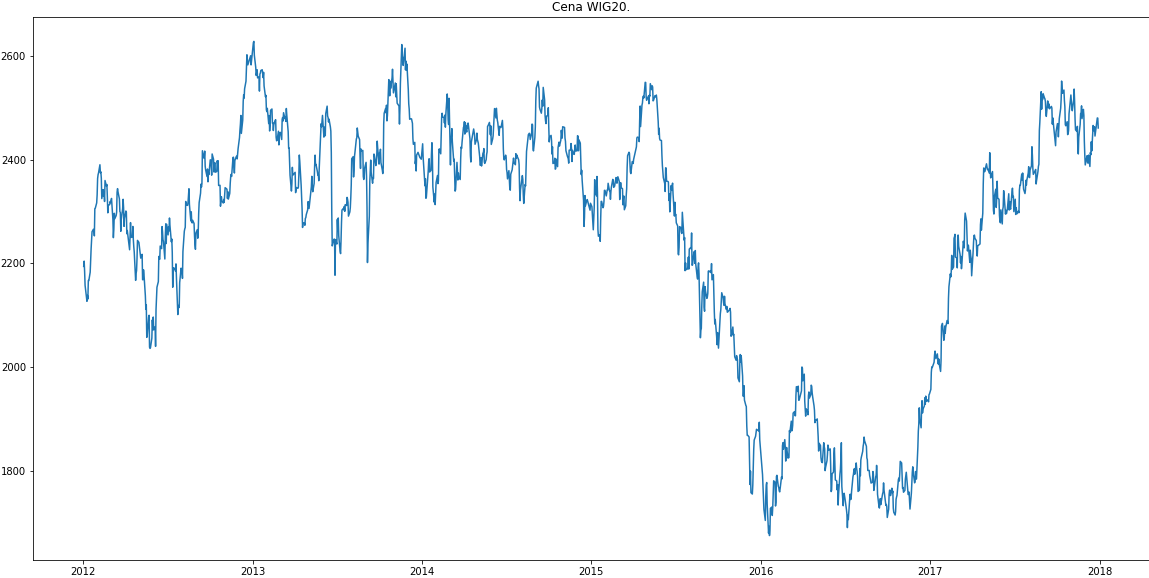
\includegraphics[width=\textwidth,height=\textheight,keepaspectratio]{wig20_cena.png}
    \caption{Zmiana notowania WIG20 w czasie.}
    \label{fig:cena_wig20}
\end{figure}

\subsection{Symulacja trajektorii WIG20.}

Zasymulowaliśmy przyszłe trajektorie WIG20 od dziś do końca roku dobierając odpowiednio zmienność i dryft na podstawie danych historycznych. Do określenia parametrów symulacji, używamy danych z okresu 2016-01-01 - 2016-12-31. Otrzymaliśmy 
\begin{align*}
\mu = 0.0648 \\ 
\sigma = 0.1900    
\end{align*}

Próbowaliśmy także danych z innych okresów: na dwa lata do tyłu, pięć lat, dziesięć lat. Te zmiany nie miały znaczącego wpływu na rezultaty w późniejszych częściach projektu.

Przyjmujemy że cena indeksu zmienia się według wzoru:
$$ dS = \mu S dt  + \sigma S dX $$

Wykres \ref{fig:pred_wig20} przedstawia chmurę tysiąca wygenerowanych trajektorii. 
Wykres \ref{fig:pred_wig20_q} przedstawia chmurę tysiąca wygenerowanych trajektorii wraz z liniami kwantylowymi. 
\\ 
Możemy zauważyć, że trajektoria podobna do prawdziwej w naszym modelu miała niewielkie prawdopodobieństwo wystąpienia (ok. 10\%). Staje się to zrozumiałe po spojrzeniu na kurs WIGu w szerszej perspektywie - wykres \ref{fig:cena_wig20}. Rok 2016 skończył się ceną zbliżoną do początkowej, w 2015 cena w skali roku spadała, a w roku 2017 mieliśmy spory wzrost ceny. Było to nie do przewidzenia modelem zakładającym, że rozkład zwrotów będzie taki jak w poprzednim roku czy kilku poprzednich. Na wykresie intuicyjnie widać, że w 2017 roku dzieje się to samo co w 2015, ale 'w górę' zamiast 'w dół'.

\begin{figure}[htp]
    \centering
    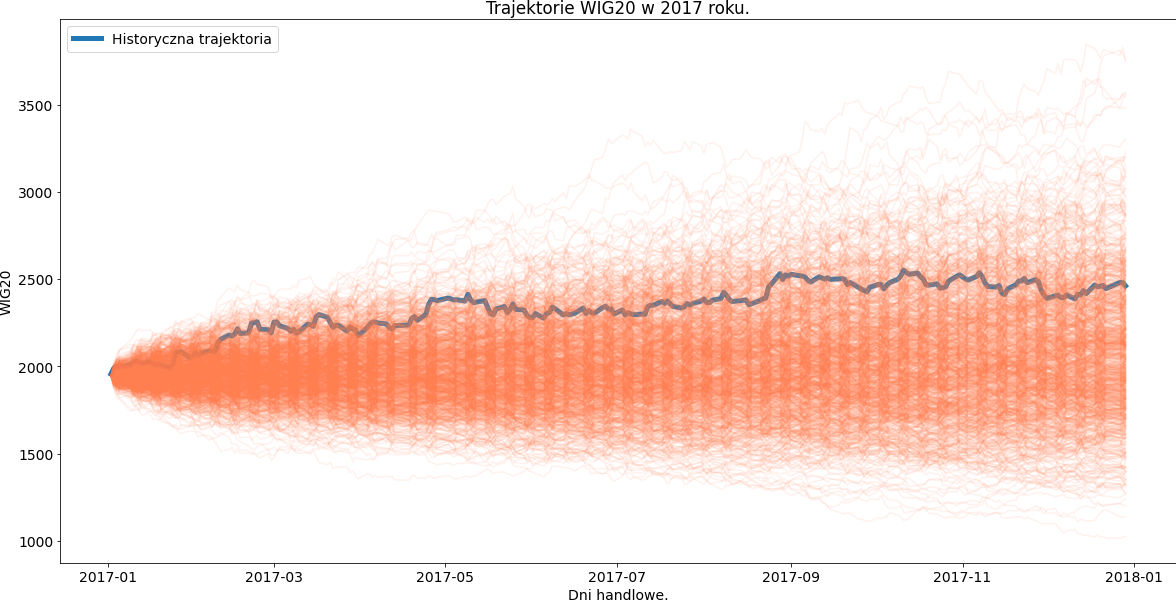
\includegraphics[width=\textwidth,height=\textheight,keepaspectratio]{trajektorie_wig20_predykcje_2017.png}
    \caption{Chmura tysiąca wygenerowanych trajektorii przyjmując dynamikę geometrycznego ruchu Browna.}
    \label{fig:pred_wig20}
\end{figure}

\begin{figure}[htp]
    \centering
    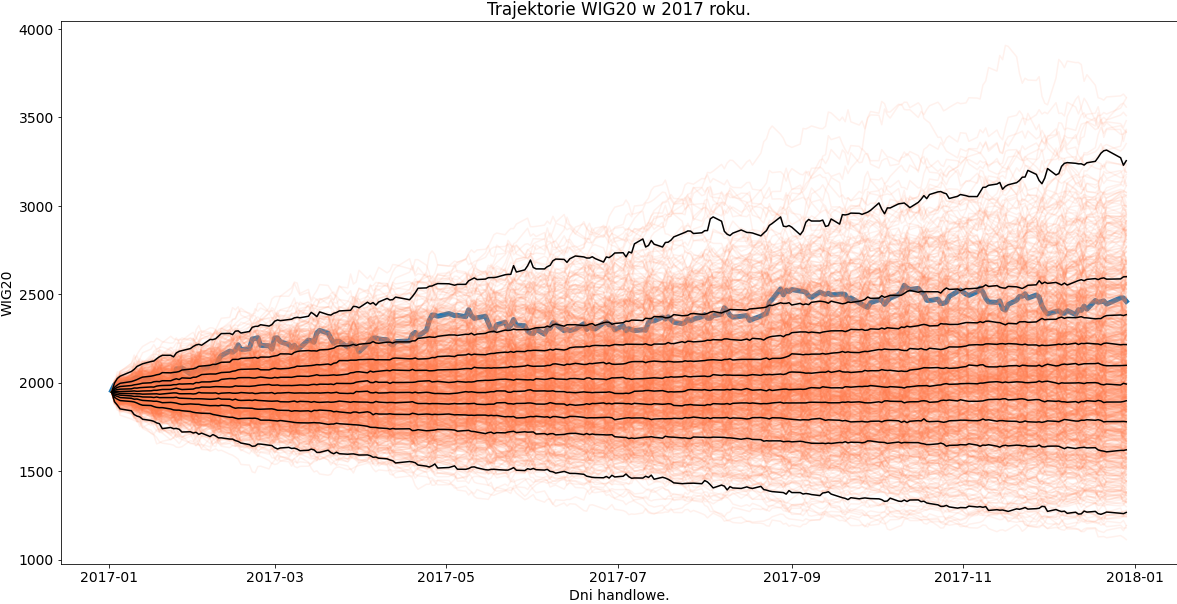
\includegraphics[width=\textwidth,height=\textheight,keepaspectratio]{trajektorie_wig20_predykcje_2017_kwantyle.png}
    \caption{Chmura tysiąca wygenerowanych trajektorii plus linie kwantylowe.}
    \label{fig:pred_wig20_q}
\end{figure}
\newpage
\subsection{Histogramy zwrotów dziennych.}
Następnie porównaliśmy histogramy historycznych zwrotów dziennych z histogramami z wygenerowanych trajektorii, które zamieściliśmy na wykresach \ref{fig:hist_wig20_true} i \ref{fig:hist_wig20_pred}. Średnie i odchylenia standardowe są podane tam w ujęciu rocznym. Widzimy, że średnia z rzeczywistych danych jest znacznie większa niż z danych wygenerowanych. Odchylenie standardowe jest natomiast mniejsze w danych rzeczywistych niż wygenerowanych. Wytłumaczyć to zjawisko można tak samo jak w poprzednim akapicie. 

\begin{figure}[H]
    \centering
    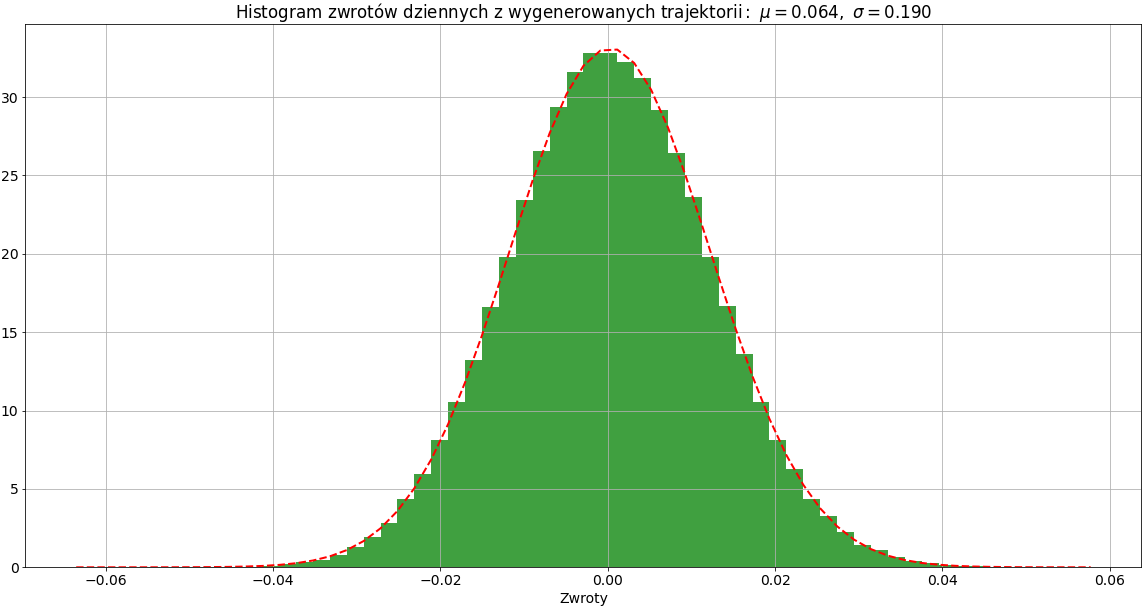
\includegraphics[width=\textwidth,height=\textheight,keepaspectratio]{hist_wig20_predykcje.png}
    \caption{Histogram zwrotów dziennych z wygenerowanych trajektorii.}
    \label{fig:hist_wig20_pred}
\end{figure}

\begin{figure}[H]
    \centering
    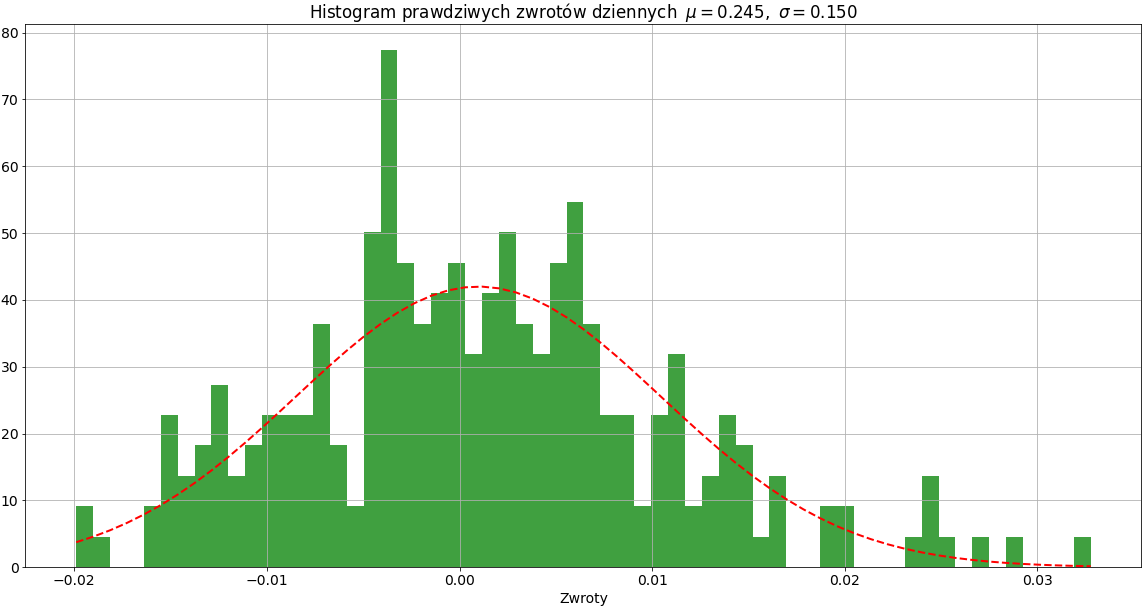
\includegraphics[width=\textwidth,height=\textheight,keepaspectratio]{hist_wig20_prawdziwe.png}
    \caption{Histogram historycznych zwrotów dziennych.}
    \label{fig:hist_wig20_true}
\end{figure}

\subsection{Standardy oraz KID dla opcji na GPW.}

Standardy opcji:
\begin{itemize}
        \item  zawsze są dostępne opcje wygasające co miesiąc przez najbliższe 3 miesiące oraz kończące się w trzech następnych miesiącach kończących kwartały (III, VI, IX, XII)
    \item  notowania prowadzi się w punktach indeksowych; jeden punkt jest wart 10 PLN
    \item po wygaśnięciu danej serii opcji wprowadza się nowe:
    \begin{itemize}
        \item  wygasające po kwartale (jedne na cenę równą aktualnej, 8 tańszych i 8 niższych)
        \item  wygasające po miesiącu na cenę równą aktualnej
        \item  dodatkowo po wygaśnięciu akcji w miesiącach kończących kwartały wprowadza się opcje wygasające po roku (jedne na cenę równą aktualnej, 4 tańsze i 4 droższe)
        \item  dodatkowo uzupełnia się rynek odpowiednimi seriami tak aby były:
        \begin{itemize}
            \item odległe o miesiąc: 16 o cenie niższej niż obecna i 16 o cenie wyższej
            \item odległe o 2 i 3 miesiące: 8 o cenie niższej niż obecna i 8 o cenie wyższej
            \item o najdalszym terminie wykonania: 4 o cenie niższej niż obecna i 4 o cenie wyższej
        \end{itemize}
        \item kolejne ceny wykonania ustala się zgodnie z pkt 1 "Standardu..." - tej tabeli nie będziemy tu zamieszczać
    \end{itemize}
    \item premią nazywa się koszt nabycia opcji.
\end{itemize}
Powyższe informacje staną się istotne w ostatniej części, gdzie używamy różnych opcji do zabezpieczania portfela. W tamtych rozważaniach używamy jedynie takich opcji, które zgodnie z powyższymi informacjami były w danym momencie dostępne na rynku.
\subsection{Wstępna analiza payoffu z różnych opcji}
Żeby badać opcje zapadające w grudniu, musimy wiedzieć jakie serie opcji o takiej zapadalności były dostępne w styczniu. Jest to 9 serii opcji o cenie wykonania zależnej od kursu indeksu pod koniec grudnia (jedna o porównywalnej, 4 o cenie wykonania niższej i 4 o wyższej). Grudniowy kurs indeksu można zaokrąglić do 1900, więc dostępne są opcje o striku od 1500 do 2300, co 100.\\
Poniżej prezentujemy przewidywany payoff kilku wybranych opcji. Dla czytelności histogramy przedstawiają jedynie rozkład payoffu gdy jest on dodatni, zaś prawdopodobieństwo, że jest on zerowy jest podane nad histogramami.\\
Zauważmy, że dla opcji call i put o tym striku te wartości sumują się do 1. Jest to oczywiste - jedna z opcji wykonuje się dokładnie wtedy gdy cena indeksu jest poniżej ceny wykonania, zaś druga w przeciwnym wypadku. Gdyby cena aktywa była dokładnie równa strikowi opcji, payoff obydwu byłby równy 0, ale ponieważ traktujemy cenę w danym czasie jako ciągła zmienną losową, to prawdopodobieństwo takiego zdarzenia jest równe 0.
\begin{figure}[htp]
    \centering
    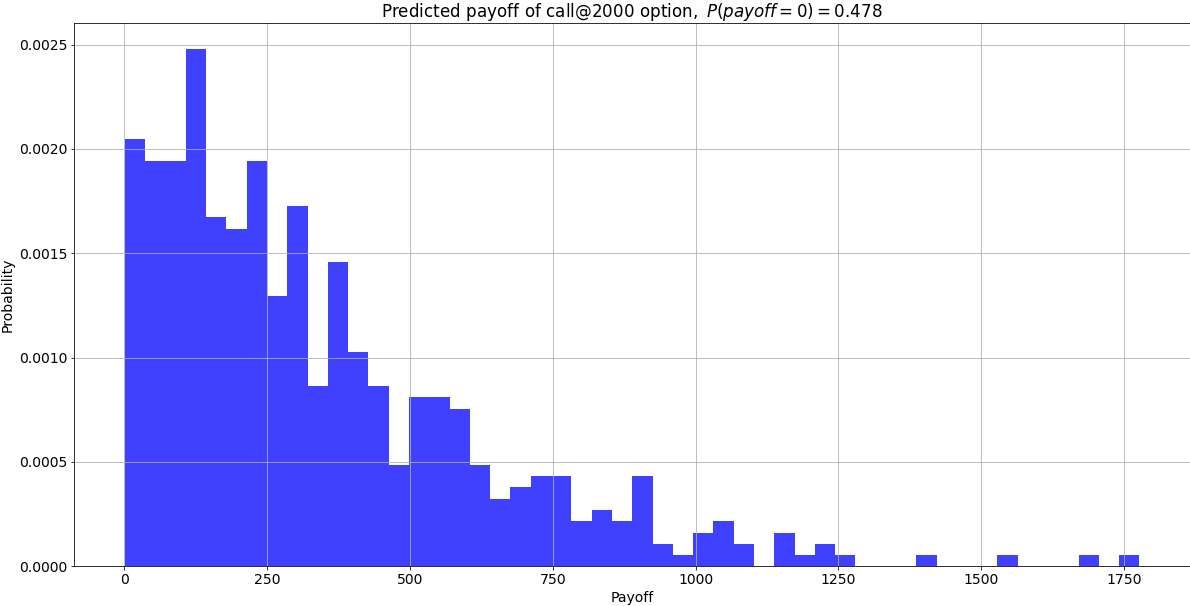
\includegraphics[width=\textwidth,height=\textheight,keepaspectratio]{payoff_call_2000.png}
    \caption{Histogram payoffu z opcji EC@2000.}
    \label{fig:payoff_call2000}
\end{figure}
\begin{figure}[htp]
    \centering
    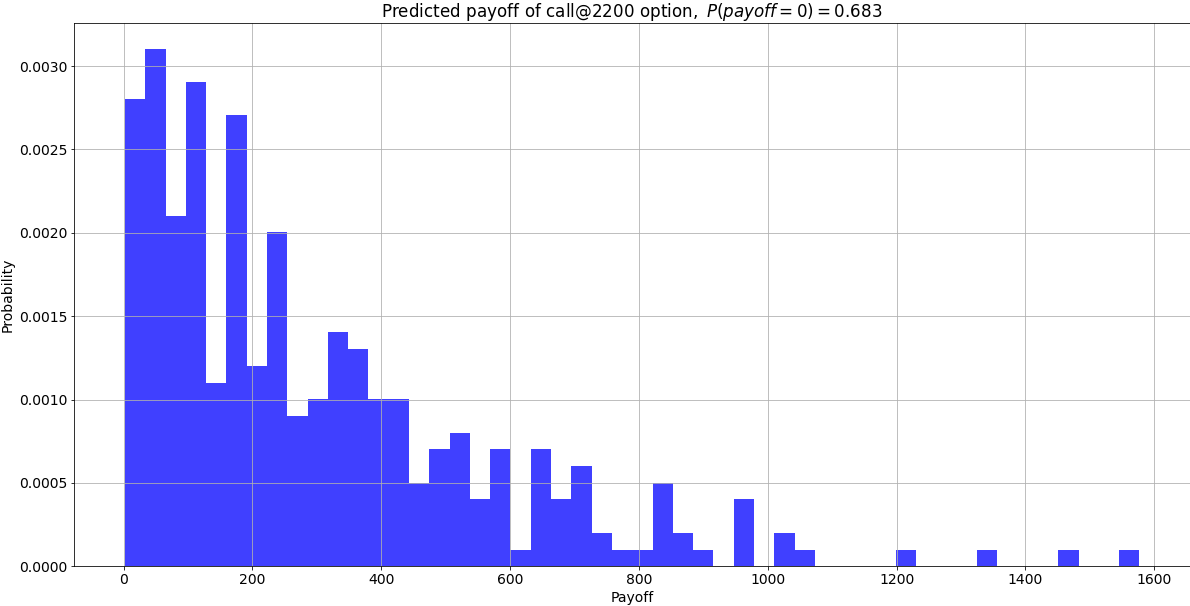
\includegraphics[width=\textwidth,height=\textheight,keepaspectratio]{payoff_call_2200.png}
    \caption{Histogram payoffu z opcji EC@2200.}
    \label{fig:payoff_call2200}
\end{figure}
\begin{figure}[htp]
    \centering
    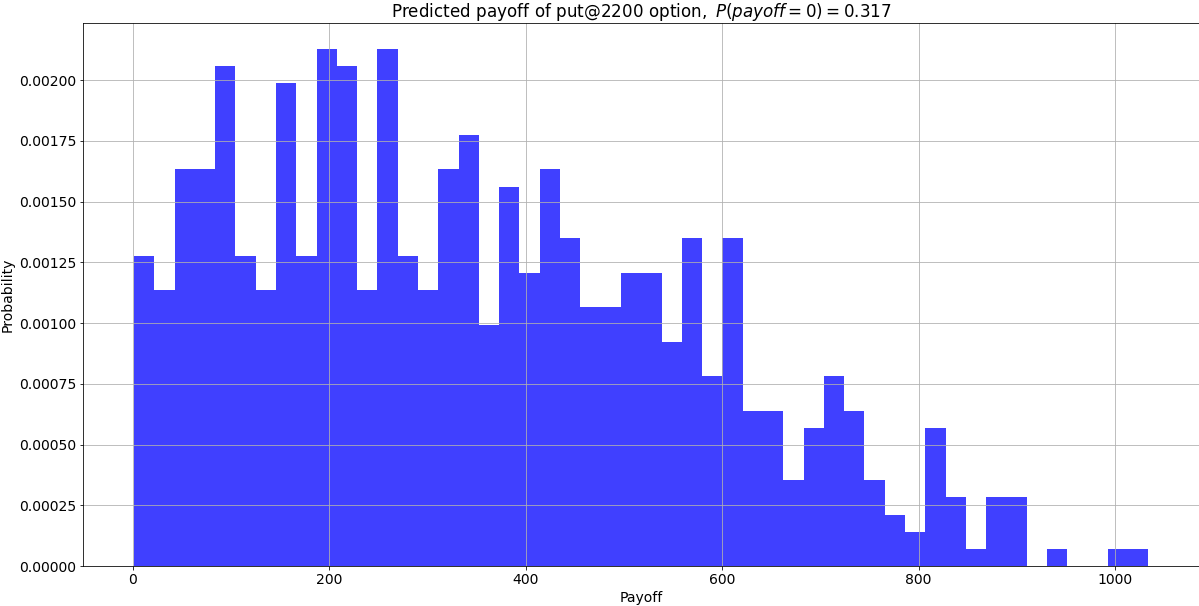
\includegraphics[width=\textwidth,height=\textheight,keepaspectratio]{payoff_put_2000.png}
    \caption{Histogram payoffu z opcji EP@2200.}
    \label{fig:payoff_put2200}
\end{figure}\\
Z obserwacji payoffów opcji call i put o striku 2200 (wykresy \ref{fig:payoff_call2200} i \ref{fig:payoff_put2200} poniżej) możemy wywnioskować najbardziej prawdopodobną cenę WIGu w grudniu - jest ona tam, gdzie najwyższe wskazanie tych histogramów. Widzimy że największe prawdopdobieństwo ma payoff około 200 z opcji put, co odpowiada cenie 2000.

\subsection{Korelacja WIG20 i KGHM}
Zasymulowaliśmy razem trajektorie WIG20 i KGHM biorąc pod uwagę silną korelację losowości ich trajektorii.  W tym celu, na podstawie danych historycznych, wyliczyliśmy macierz kowariancji . Otrzymaliśmy współczynnik korelacji: 
$$
\corr(\text{WIG20}, \text{KGHM}) = 66 \%.
$$
Następnie generowaliśmy zwroty przy użyciu dwuwymiarowego rozkładu normalnego o średniej $\mu = (\mu_{  \text{WIG20}}, \mu_{\text{KGHM}})$ i macierzy kowariancji $\Cov(\text{WIG20}, \text{KGHM}).$ Otrzymane predykcje są na wykresach \ref{fig:corr_kghm} i \ref{fig:corr_wig}.


\begin{figure}[H]
    \centering
    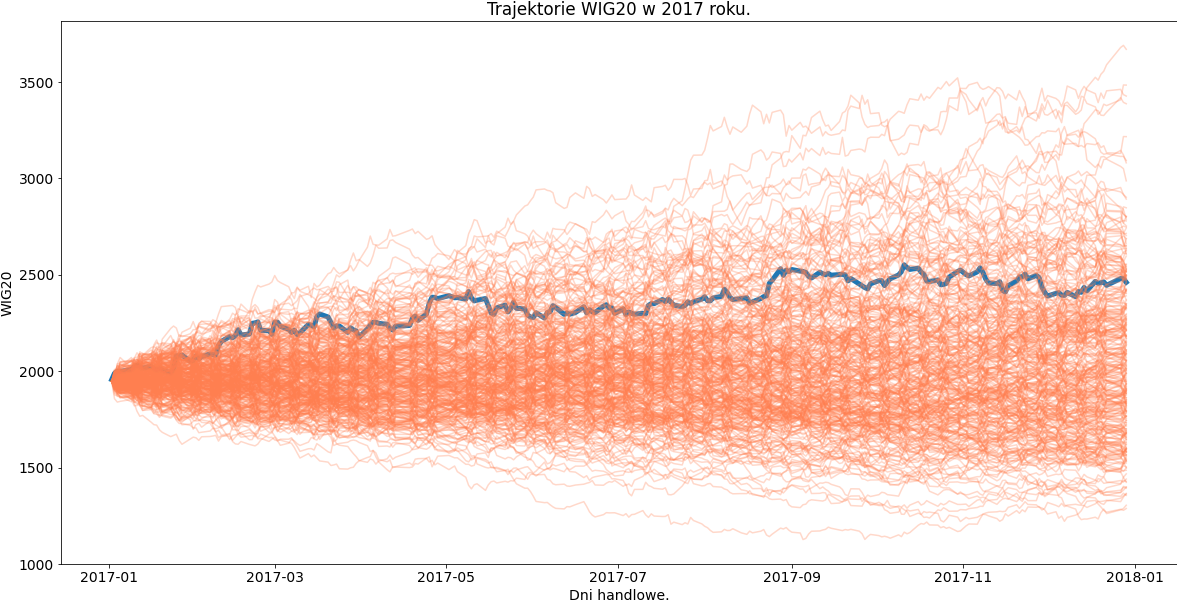
\includegraphics[width=\textwidth,height=\textheight,keepaspectratio]{corr_wig.png}
    \caption{Korelacja WIG20 i KGHM.}
    \label{fig:corr_wig}
\end{figure}

\begin{figure}[H]
    \centering
    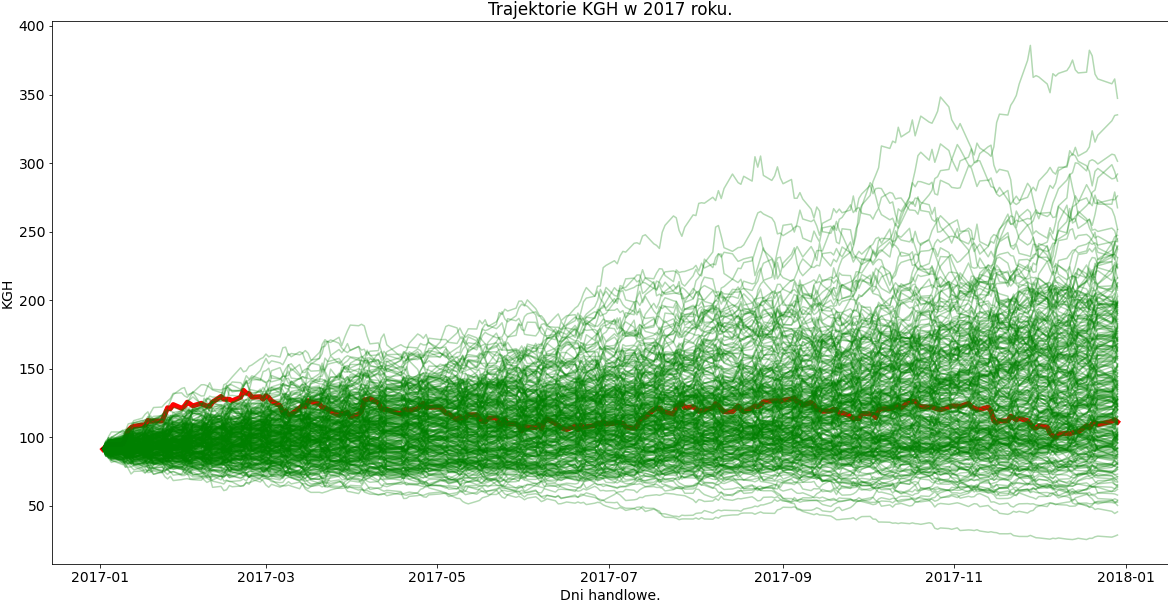
\includegraphics[width=\textwidth,height=\textheight,keepaspectratio]{corr_kghm.png}
    \caption{Korelacja WIG20 i KGHM.}
    \label{fig:corr_kghm}
\end{figure}

\subsection{Stopa wolna od ryzyka.}

Stopę wolną od ryzyka można ustalić patrząc na historyczne oprocentowanie obligacji skarbowych. 
$$
r_{2017} = 1.7\%
$$

Tutaj, \url{https://www.obligacjeskarbowe.pl/komunikaty/#year=2016}, jest napisane, że dwuletnie obligacje skarbowe miały oprocentownaie 2.1 \%. Natomiast z \url{https://pl.investing.com/rates-bonds/poland-1-year-bond-yield} wychodzi 1.7 \%. Tak małe zmiany nie miały wpływu na dalszą analizę.


\subsection{Symulacje metodą bootstrappingu.}

Porównawczo wykonaliśmy symulacje trajektorii WIG20 metodą bootstrappingu  z historycznych zwrotów. Wyniki przedstawia wykres \ref{fig:bootstrap}. Pokrywają się one z wynikami uzyskanymi przez modelowanie za pomocą geometrycznego ruchu Browna, por. wykres \ref{fig:pred_wig20}. Intuicyjnie można to uzasadnić mówiąc, że obie te metody zakładają, że przyszłe zwroty będą miały taki sam rozkład jak historyczne zwroty. Wtedy ewentualne różnice wynikające ze sposobu generowania odpowiednich próbek znikają przy dostatecznie wielu wygenerowanych trajektoriach.

\begin{figure}[htp]
    \centering
    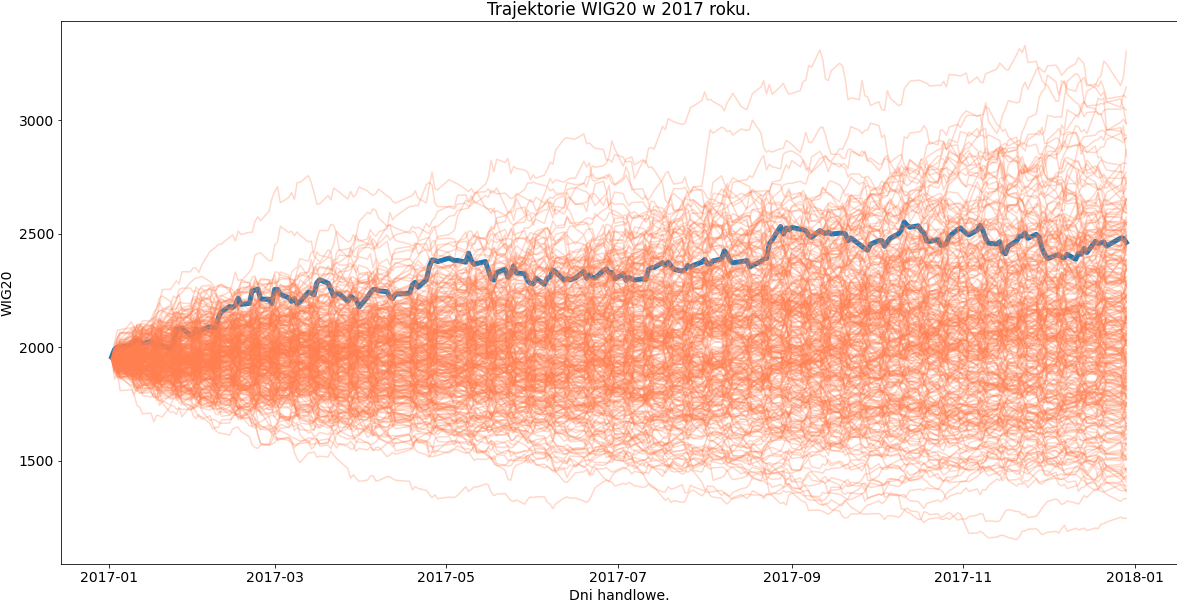
\includegraphics[width=\textwidth,height=\textheight,keepaspectratio]{bootstrapping.png}
    \caption{Trajektorie WIG20 wygenerowane metodą bootsrappingu.}
    \label{fig:bootstrap}
\end{figure}

\newpage
\section{Część A - delta hedging}
W tej części przeprowadziliśmy symulację handlowania opcjami call i put. Założenia:
\begin{itemize}
    \item Zaczynaliśmy z portfela wartego 0 złotych. 
    \item Stosowaliśmy delta hedging by zniwelować ryzyko. 
    \item Opcje na WIG20 zabezpieczaliśmy przy pomocy indeksu WIG20 i inwestycji wolnej od ryzyka - obligacji. 
    \item Ruchy indeksu modelowaliśmy geometrycznym ruchem Browna. 
    \item Dla uproszczenia nie uwzględniamy kosztów transakcji. 
\end{itemize} 

Będziemy badać portfel składający się z opcji na indeks, indeksu i pieniędzy (inwestycji wolnej od ryzyka). Skorzystamy z formuły Blacka-Scholesa na cenę opcji call. Mamy:

$$V_{call}=SN(d_1)-Ee^{-r(T-t)}N(d_2),$$
gdzie $N(x)$ jest dystrybuantą rozkładu normalnego, $S$ to obecna cena indeksu, $E$ to strike rozważanej opcji, $r$ to stopa procentowa pozbawiona ryzyka, $T$ to chwila wykonania, a $t$ to chwila obecna (wyrażane w latach). Dodatkowo,

$$d_1=\frac{log(\frac{S}{E})+(r+\frac{\sigma^2}{2})(T-t)} {\sigma \sqrt{T-t}}$$ oraz $$d_2=d_1-\sigma(T-t).$$

Nie znamy dokładnej wartości $\sigma$, więc korzystamy z tego co wyliczyliśmy na początku na podstawie danych historycznych. Dzięki call-put parity, czyli równaniu $$V_{call}+Ee^{-r(T-t)}=V_{put}+S,$$ wyliczymy cenę odpowiedniej opcji put. Korzystając z liczonych wcześniej trajektorii ceny indeksu, zbadamy rozkład zysku z naszego portfela dla różnych opcji w zależności od liczby rehedgingów.

\subsection{Świat abstrakcji}
\subsubsection{Rozkład zysku/straty z portfela zabezpieczającego.}
Przeprowadziliśmy symulację ewolucji portfela przy rehedgingach oddalonych o różną liczbę dni. Poniższy histogram przedstawia rozkład zysku z opcji call@2000. Wyniki dla różnych częstości rehedgingu są zaznaczone różnymi kolorami.
\begin{figure}[H]
    \centering
    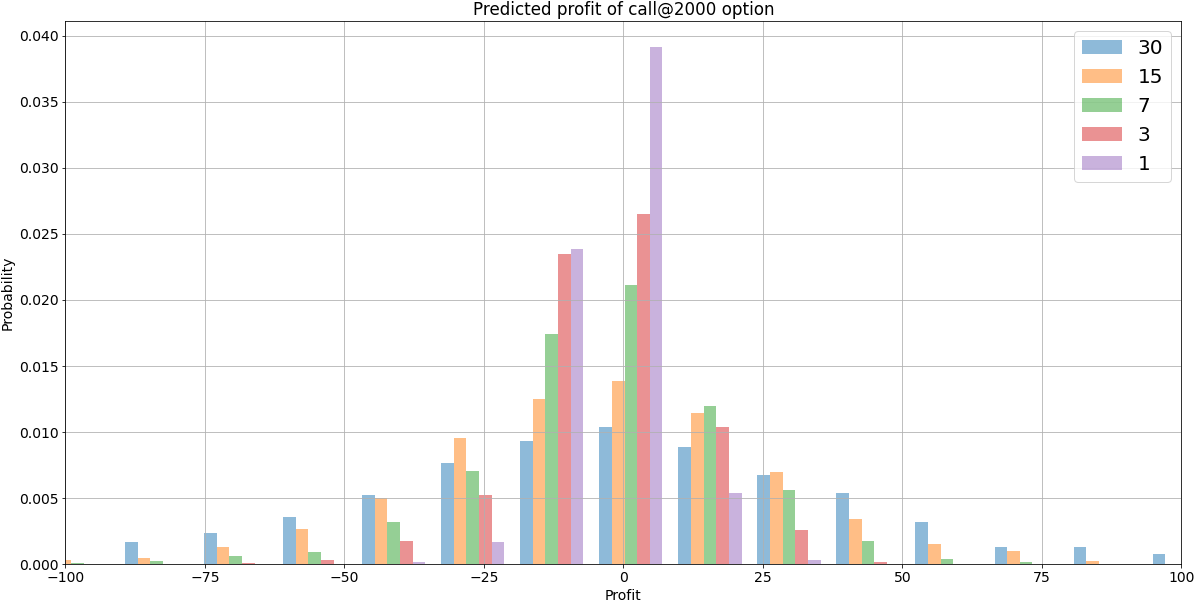
\includegraphics[width=\textwidth,height=\textheight,keepaspectratio]{multi_histogram.png}
    \caption{Zyski/straty w zależności od częstości rehedgingów dla EC@2000.}
    \label{fig:ec2000_hist_zysk}
\end{figure}
Wygodniej może być zobaczyć te informacje w formie osobnych histogramów, jak to przedstawiamy poniżej \ref{fig:hist_all}.\\
\begin{figure}[H]
    \centering
    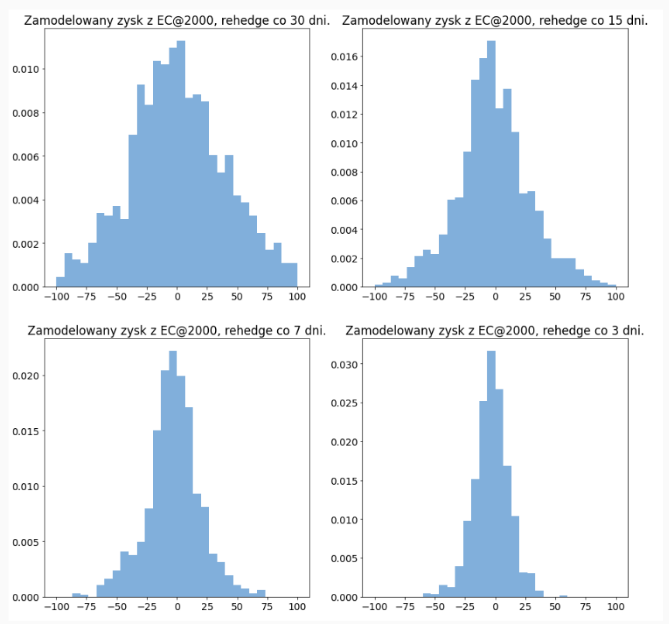
\includegraphics[width=\textwidth,height=\textheight,keepaspectratio]{hist_rehedge_freq.png}
    \caption{Zyski/straty w zależności od częstości rehedgingów dla EC@2000.}
    \label{fig:hist_all}
\end{figure}

Widzimy, że jest to rozkład scentrowany w zerze, którego wariancja zmniejsza się wraz z odstępem między kolejnymi rehedgingami. Przy codziennym rehedgingu odchylenie standardowe wynosi około 8.8.\\
\subsubsection{Kwantyle zysku/straty.}
Na wykresie przedstawiającym kwantyle zysku (\ref{fig:kwantyle}) w zależności od liczby dni między rehedgingami możemy zauważyć kilka rzeczy:

\begin{itemize}
    \item Prawie nigdy nie otrzymujemy zysku/straty o wartości bezwzględnej przekraczającej 100.
    \item Przy codziennym rehedgingu z 98\% prawdopodobieństwem wartość bezwzględna naszego zysku/straty nie przekracza 25.
    \item Gdyby dało się robić rehedging częściej niż raz dziennie, wszystkie linie powinny zbiegać do punktu (0,0).
\end{itemize}
\begin{figure}[H]
    \centering
    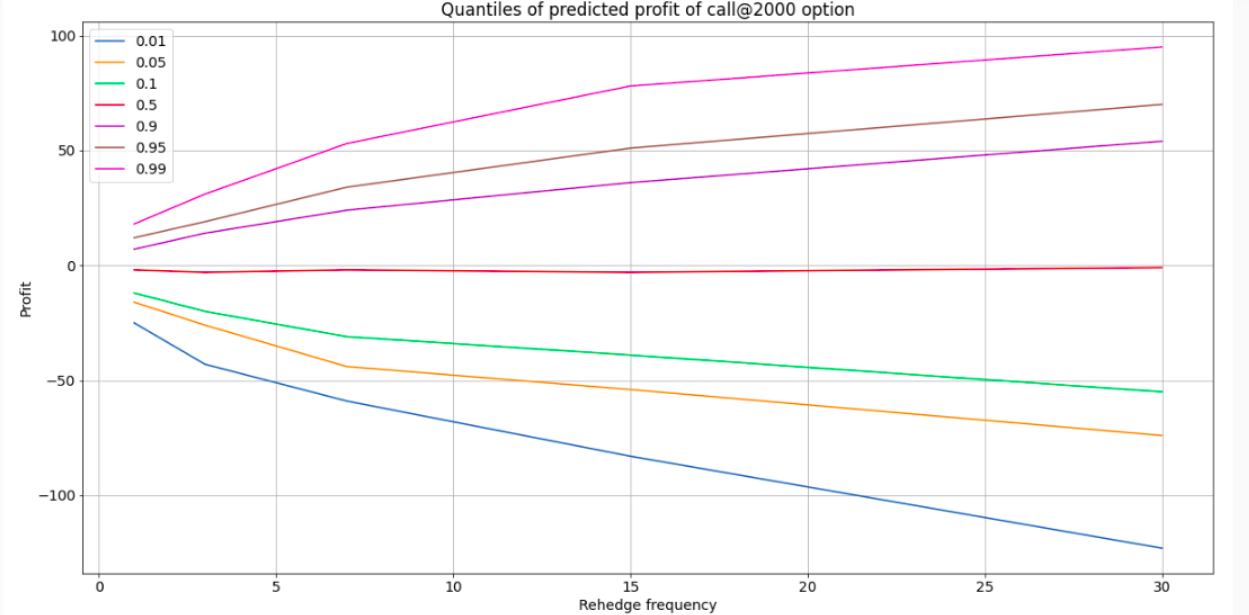
\includegraphics[width=\textwidth,height=\textheight,keepaspectratio]{kwantyle.png}
    \caption{Zyski/straty w zależności od częstości rehedgingów dla EC@2000.}
    \label{fig:kwantyle}
\end{figure}
\subsubsection{Premia za ryzyko.}
Z powyższych obserwacji oraz bardziej wnikliwej analizy obliczonych kwantyli możemy oszacować premię jakiej oczekiwalibyśmy od nabywcy naszej opcji. Przy codziennym rehedgingu z prawdopodobieństwem 0.1 mamy zysk większy niż -13, zaś z prawdopodobieństwem 0.05 większy niż -17. Okazuje się, że jeśli nabywca naszej opcji będzie przyjmował $\sigma$ większe o 10\% od naszego, to będzie skłonny zapłacić dodatkowe 9\% ceny opcji (ok. 14 zł), co sprawia, że z prawdopodobieństwem ponad 90\% wyjdziemy z całego procesu z zyskiem. Dodatkowo, jeśli ktoś przyjmuje $\sigma$ większe o 12\%, to będzie skłonny zapłacić za opcję 11\% więcej niż jej pierwotna cena, tym samym zmniejszając nasze prawdopodobieństwo straty pieniędzy poniżej 5\%.\\
Otrzymanie $\sigma$ tak różniącego się od naszego jest możliwe - wystarczy patrzeć na dane z nieco innego okresu z przeszłości żeby otrzymać parametry różniące się o 10-15\%.

\subsection{Świat rzeczywisty}
\subsubsection{Faktyczne zyski/straty z portfela zabezpieczającego.}
Wykres \ref{fig:ec2000_zyski} przedstawia zyski w
 zależności od częstości rehedgingów dla EC@2000 na faktycznych notowaniach z 2017 roku. Widzimy, że zazwyczaj zyski mieszczą się w przedziale 5 - 15 zł. Przy zbyt rzadkich rehedgingach tracimy tę własność.
 \newline
\begin{figure}[htp]
    \centering
    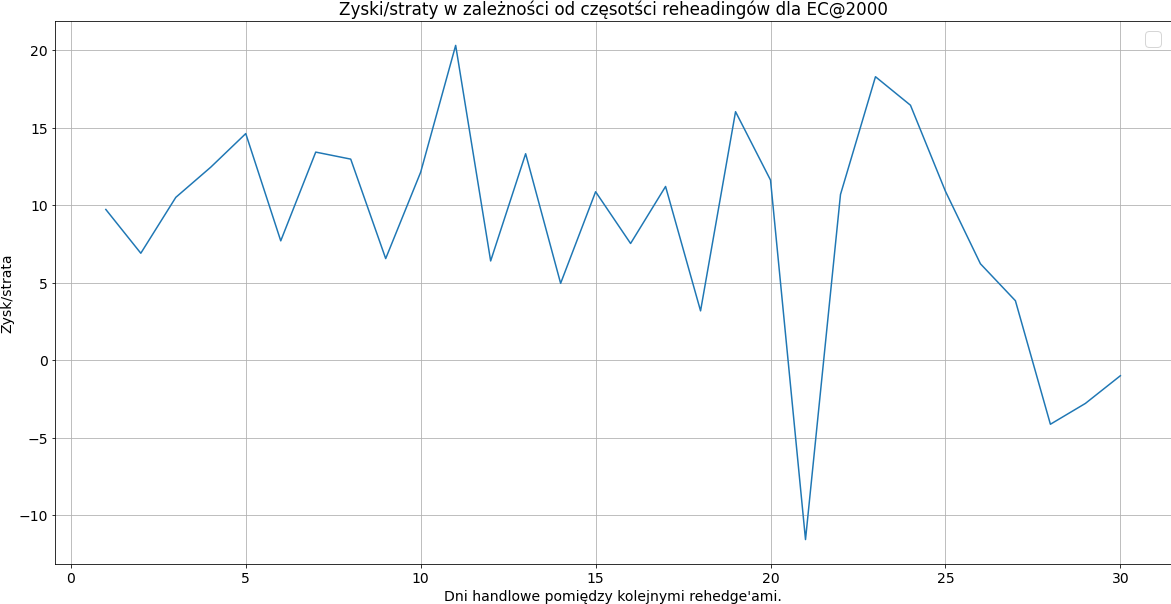
\includegraphics[width=\textwidth,height=\textheight,keepaspectratio]{EC@2000_zyski_od_czestosci_reheadge.png}
    \caption{Zyski/straty w zależności od częstości rehedgingów dla EC@2000.}
    \label{fig:ec2000_zyski}
\end{figure}

\subsubsection{Skład portfela w czasie.}

Wykres \ref{fig:sklad_portfela} przedstawia skład portfela w czasie dla EC@2000 i EP@2000 przy rehedgingach co 10 dni handlowych.  Wykres zmiany $\Delta_{call}(t)$ i $\Delta_{put}(t) $ zgadza się ze wzorami teoretycznymi
$$
\Delta_{call}(t) = N(d_1),
$$
$$
\Delta_{put}(t) = N(d_1) - 1.
$$
Wypłaszczenie, jakie obserwujemy od września, wynika z faktu, że cena indeksu przekroczyła strike i jest stale powyżej strike'u. Zatem prawie na pewno opcja call zostanie wykonana, więc w portfelu trzymamy jedną jednostkę indeksu, żeby zabezpieczyć wykonanie opcji call.  Podobnie rozumując, opcja put prawie na pewno nie zostanie wykonana.
\begin{figure}[htp]
    \centering
    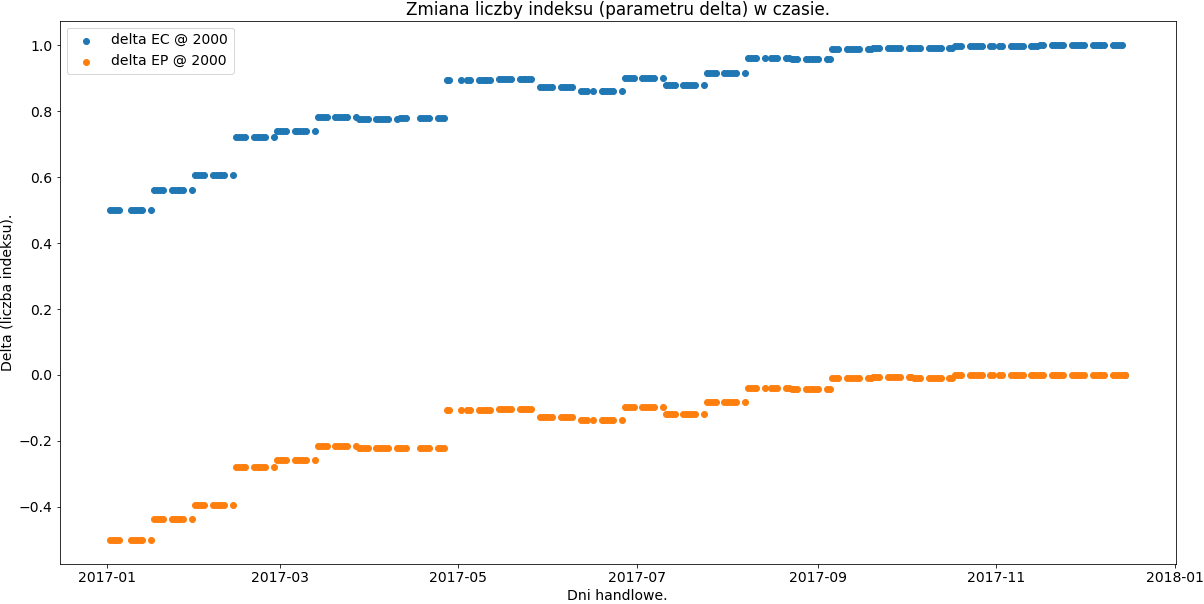
\includegraphics[width=\textwidth,height=\textheight,keepaspectratio]{sklad_portfela_w_czasie.png}
    \caption{Zmiana liczby indeksu w czasie.}
    \label{fig:sklad_portfela}
\end{figure}

\subsubsection{Narastająco zysk/strata w czasie.}

Wykres \ref{fig:narastajaco_wartosc} przedstawia narastająco zysk/stratę dla EC@2000 i EP@2000 przy rehedgingach co 10 dni handlowych. Widzimy, że wartość portfela nie zależy od rodzaju opcji.  Zgadza się to ze wzorami teoretycznymi. 

\begin{figure}[H]
    \centering
    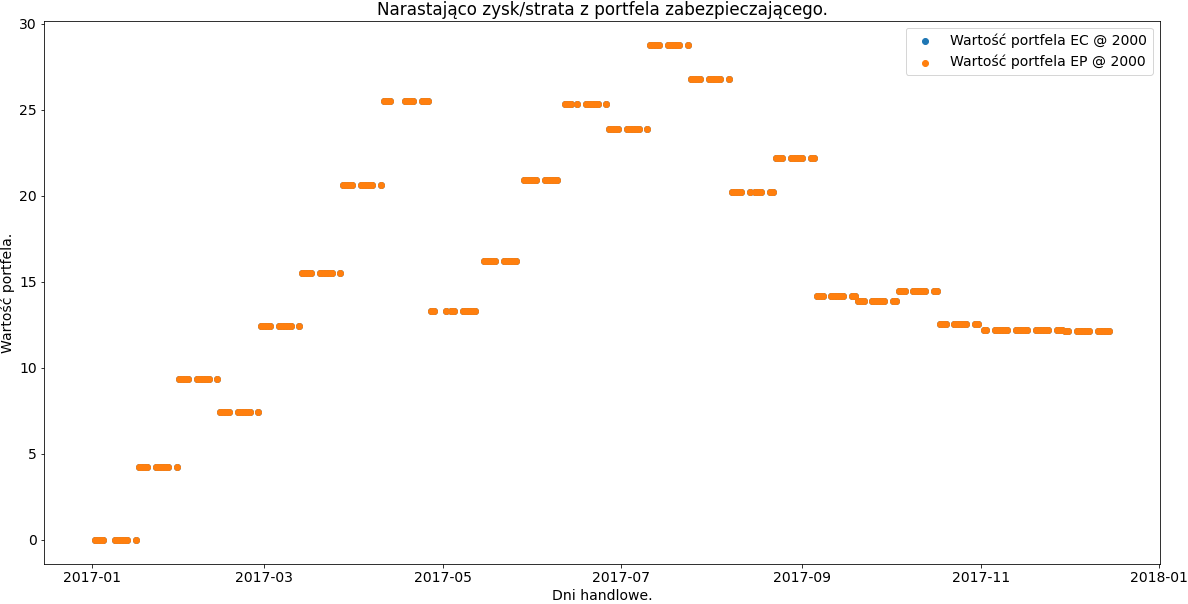
\includegraphics[width=\textwidth,height=\textheight,keepaspectratio]{narastajaco_zysk_delta_hedge.png}
    \caption{Narastająco zysk/strata z portfela zabezpieczającego.}
    \label{fig:narastajaco_wartosc}
\end{figure}

\section{Część B - delta i gamma hedging.}
\subsection{Idea + wzory.}
W tej części zakładamy dodatkowo, że każda transakcja jest obarczona pewnym kosztem. Między innymi oznacza to, że nie możemy już bezstresowo zwiększać liczby rehedgingów. W tym wypadku chcielibyśmy ograniczyć je do minimum, nie tracąc jednak kontroli nad zmiennością portfela. W tym celu wprowadzamy gamma hedging, czyli zerowanie drugiej pochodnej portfela względem ceny akcji. 

Do zabezpieczania portfela będziemy używać indeksu i opcji binarnych. Zakładamy, że koszt każdej transakcji wynosi 4\% jej wartości. 

\subsection{Delta-hedging z kosztami transakcyjnymi.}

By postawić dalsze wynik w perspektywie, dobrze jest zobaczyć najpierw jak zmieniają się rezultaty otrzymane przez delta hedging po dodaniu kosztów transakcyjnych (wykres \ref{fig:deltazkosztami}).

\begin{figure}[H]
    \centering
    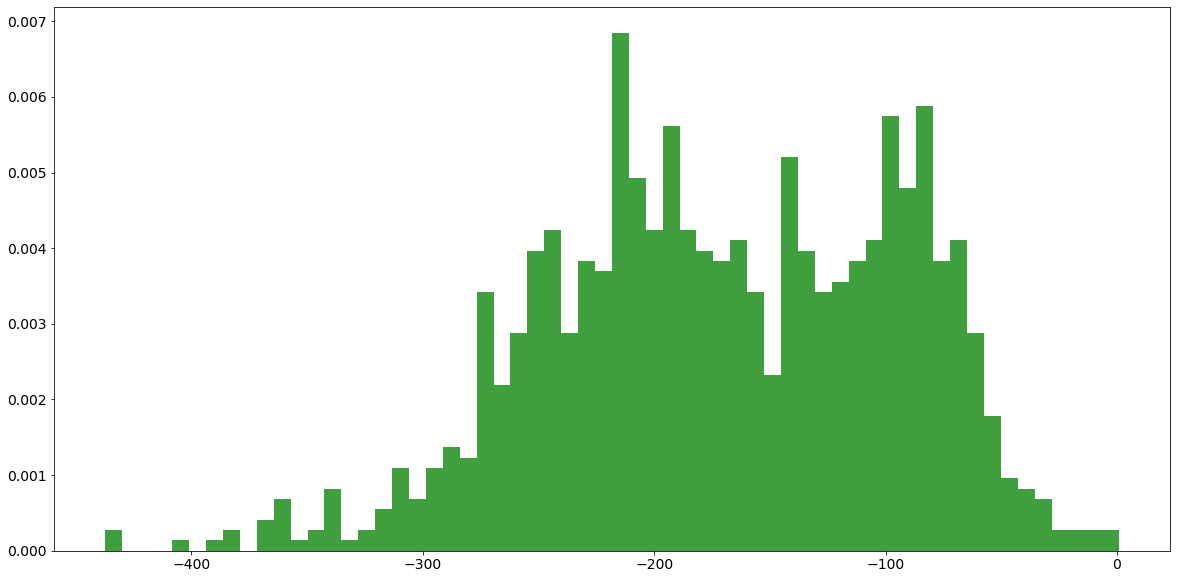
\includegraphics[width=\textwidth,height=\textheight,keepaspectratio]{deltazkosztami.png}
    \caption{Histogram zysków przy delta hedgingu co 30 dni z kosztami transakcyjnymi.}
    \label{fig:deltazkosztami}
\end{figure}

Większość obserwacji znajduje się w przedziale pomiędzy -300 a 0. Przy delta hedgingu bez kosztów odchylenia były na poziomie kilkudziesięciu punktów, więc widać, że sytuacja znacząco się pogorszyła. 

\subsection{Zwykły gamma hedging (i problemy z nim związane).}

Rozważamy europejską opcję call z ceną wykonania 2000. Do zabezpieczenia portfela będziemy kupować/sprzedawać pewną liczbę indeksu i binarnej opcji put z tą samą ceną i czasem wykonania. Nasz portfel wygląda więc następująco:
$$
\Pi = V_1 - aS - bV_2
$$
Chcemy mieć $\frac{\partial \Pi}{\partial S} = 0$ oraz $\frac{\partial^2 \Pi}{\partial S^2} = 0$. Oznaczając $\Delta_1 = \frac{\partial V_1}{\partial S}$, $\Delta_2 = \frac{\partial V_2}{\partial S}$, $\Gamma_1 = \frac{\partial^2 V_1}{\partial S^2}$, $\Gamma_2 = \frac{\partial^2 V_2}{\partial S^2}$ łatwo więc wyliczyć 
$$
b = \frac{\Gamma_1} {\Gamma_2} \hspace{1cm} a = \Delta_1 - b\Delta_2
$$
Naiwny gamma hedging będzie więc polegał na tym, że z określoną częstością będziemy wyliczać parametry a i b i kupować odpowiednią liczbę akcji/opcji. Poniższy wykres przedstawia efekt takiego działania przy rehedgingach co 30 dni.


\begin{figure}[htp]
    \centering
    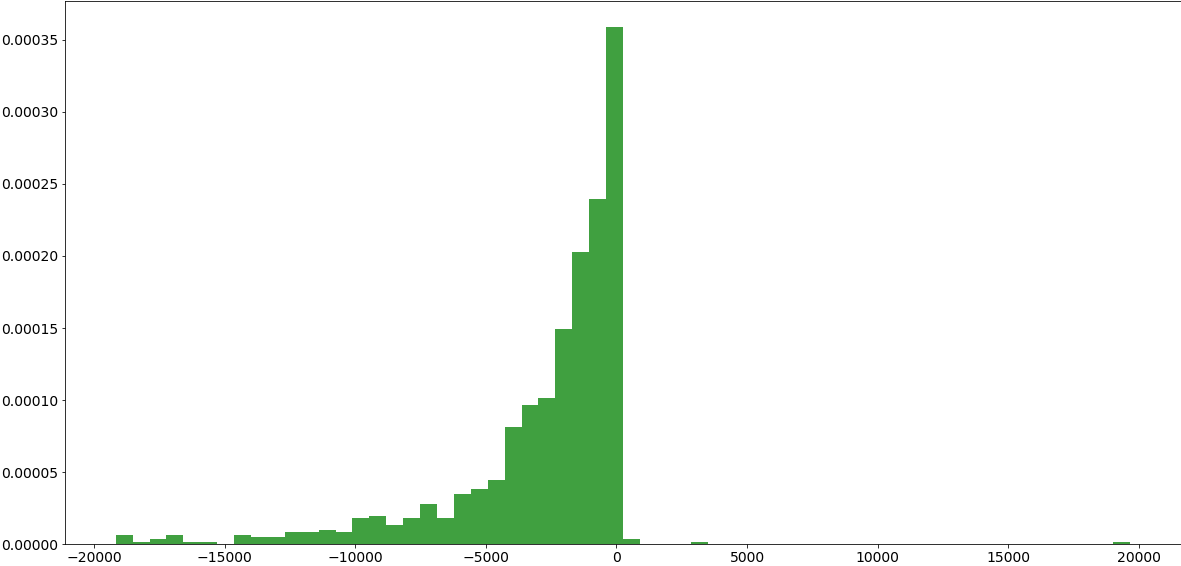
\includegraphics[width=\textwidth,height=\textheight,keepaspectratio]{hist_nawiny_gamma_hedging(1).png}
    \caption{Histogram zysków przy zastosowaniu gamma-hedgingu co 30 dni}
    \label{fig:hist_naiwny_gamma_hedging}
\end{figure}

Widać, że większość obserwacji rzeczywiście skupia się wokół 0. Brak obserwacji przynoszących istotny zysk jest spodziewany, bo po to właśnie robimy hedging, żeby zminimalizować ryzyko, a minimalizacja ryzyka będzie się wiązać z minimalizacją zysków/strat. Wysokie straty pojawiające się przy części obserwacji nie są spowodowane nieskutecznością hedgingu, a kosztami transakcyjnymi. Pojawia się dużo obserwacji przynoszących wysoką stratę, na poziomie kilkunastu tysięcy, a nawet kilka niewidocznych na wykresie, które przyniosły stratę rzędu kilkuset tysięcy. Jest to spowodowane tym, że gdy $\Gamma_2$ jest bardzo mała, to musimy kupić ogromną liczbę opcji binarnych, co generuje wysoki koszt transakcji. Stąd należy wnioskować, że stosując gamma hedging trzeba zachować pewne środki ostrożności. 


\subsection{Gamma hedging - podejście 2.}

Jednym z powodów, dla których $\Gamma_2$ może być bliska 0, jest to, że cena wykonania opcji binarnej jest daleka od aktualnej ceny akcji, przez co wartość opcji binarnej jest równa 0 lub 1 i niewielkie wahania ceny akcji nie powodują istotnej zmiany. To sugeruje, że gdybyśmy byli w stanie dostosować cenę wykonania opcji tak, żeby była bliższa aktualnej cenie akcji, powinniśmy otrzymać lepsze rezultaty.

W tym celu będziemy zmieniać opcje w trakcie roku. Konkretnie będziemy kupować binarne opcje put na miesiąc z ceną wykonania równą aktualnej cenie akcji. 

\begin{figure}[htp]
    \centering
    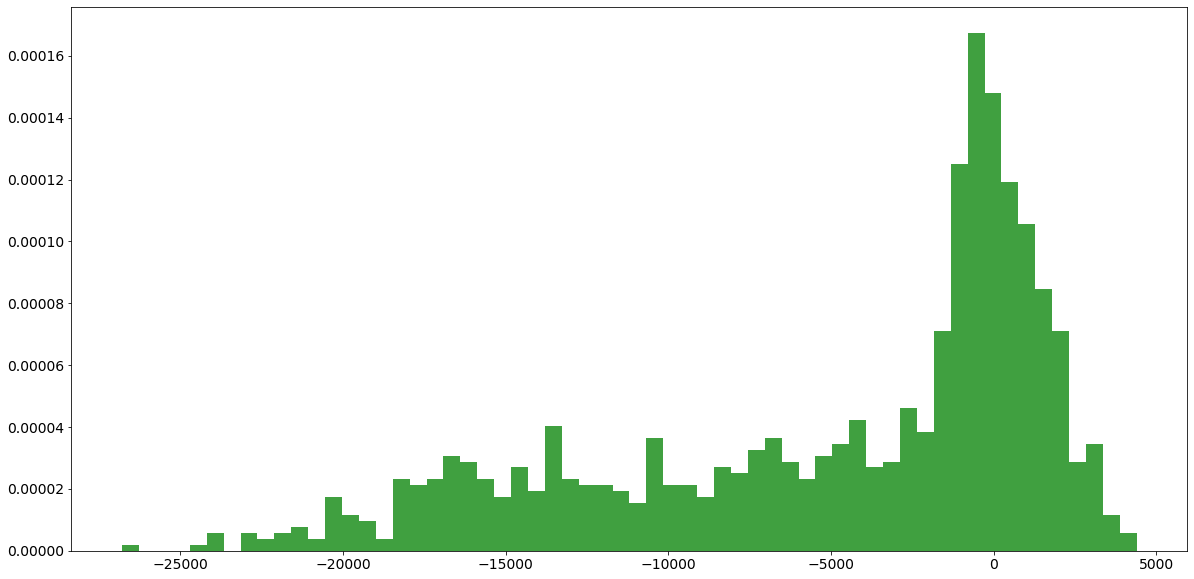
\includegraphics[width=\textwidth,height=\textheight,keepaspectratio]{gammarestock30.png}
    \caption{Histogram zysków przy wymianie opcji co miesiąc}
    \label{fig:gammarestock}
\end{figure}

Tutaj oglądamy już kompletny wykres - to znaczy takie podejście wyeliminowało skrajne przypadki dające w poprzednim podejściu stratę rzędu kilkuset tysięcy. Widać jednak, że sytuacja wciąż jest daleka od idealnej i straty na poziomie kilkunasty tysięcy są nadal na porządku dziennym. Można też zauważyć, że tutaj obserwujemy istotny zysk dla części trajektorii. Nie jest to bardzo zaskakujące - jeśli nadal musimy kupować duże ilości opcji, to w części przypadków przyniosą one pewien zysk, a jako że opcje rozliczane są tutaj co miesiąc (a nie jeden raz na końcu jak w poprzednim przypadku), to zysk ten może być stosunkowo duży. 
Choć jest lepiej niż poprzednio, to nadal trudno nazwać taki rezultat zadowalającym - w szczególności jest znacznie gorszy niż sam delta hedging.

\subsection{Gamma hedging - do trzech razy sztuka.}

Skoro minimalizacja gammy w sposób jak wyżej się nie powiodła, to spróbujmy zminimalizować ją nieco bardziej brutalnie. Gdy popatrzymy na wzory 
$$
\frac{\partial^2 \Pi}{\partial S^2} = \Gamma_1 - b\Gamma_2 \hspace{1cm} b = \frac{\Gamma_1}{\Gamma_2}
$$

można zaobserwować dwie rzeczy:
\begin{itemize}
    \item 1. Gdy $\Gamma_1$ i $\Gamma_2$ są małe, to druga pochodna portfela jest mała - to oznacza że gamma hedging traci sens, bo jego celem jest właśnie minimalizacja drugiej pochodnej.
    \item 2. Gdy $\Gamma_1$ jest duża a $\Gamma_2$ jest mała, to liczba potrzebnych opcji binarnych jest ogromna i choć druga pochodna portfela jest wtedy istotnie niezerowa, to wyzerowanie jej jest zbyt kosztowne, żeby miało sens.
\end{itemize}
Oznacza to, że robienie gamma hedgingu wtedy, gdy $\Gamma_2$ jest mała nie ma zbyt wiele sensu. Spróbujemy więc ograniczyć się do przypadku, gdy $\Gamma_2$ jest istotnie niezerowa. W tym wypadku przez istotną niezerowość będziemy rozumieć $|\Gamma_2| > 10^{-3}$. Tam gdzie $\Gamma_2$ jest mniejsza wykonujemy jedynie delta hedging. 

\begin{figure}[H]
    \centering
    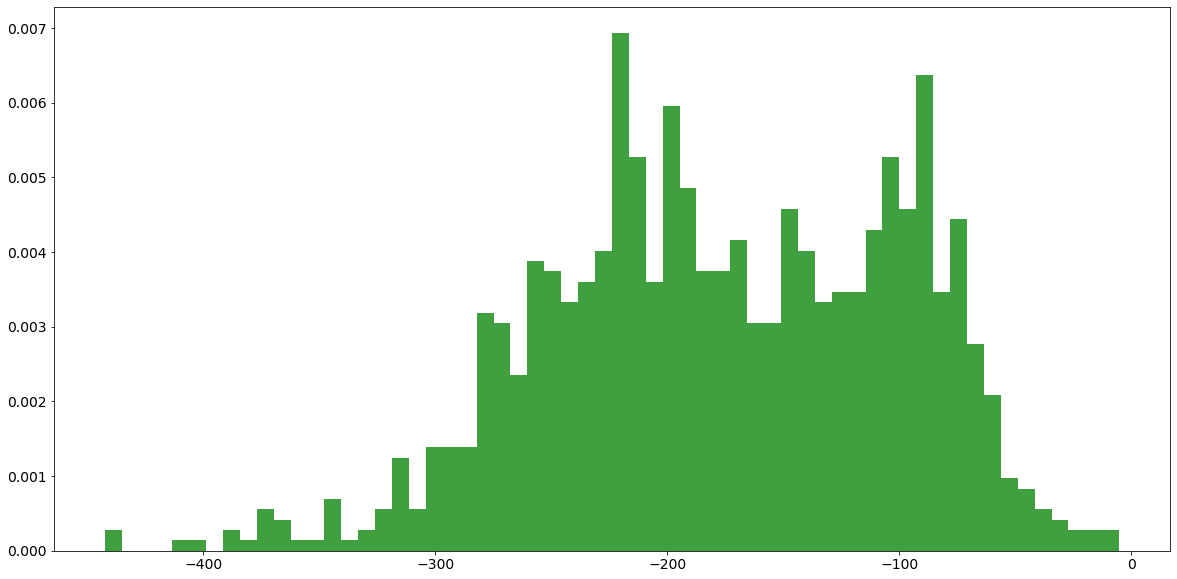
\includegraphics[width=\textwidth,height=\textheight,keepaspectratio]{gammaztolerka.png}
    \caption{Histogram zysków przy zastosowaniu hedgingu z tolerancją = 0.001}
    \label{fig:gammaztolerką}
\end{figure}

Wykres zaczął wyglądać przyzwoicie - nie mamy już wielotysięcznych strat. Problem w tym, że wykres ten nie różni się prawie niczym od przedstawionego kilka stron wcześniej delta hedgingu. Oznacza to, że przy ustawionej wyżej tolerancji gamma prawie nigdy nie była większa i cały algorytm zredukował się do zwykłego delta hedgingu. Żeby faktycznie wykorzystać zalety gamma hedgingu trzeba więc rozsądniej dobierać opcje, by ich $\Gamma$ była większa.

\subsection{Gamma hedging - tym razem na pewno się uda.}
W tej części spróbujemy rozwinąć pomysły przedstawione wcześniej. Naszym głównym celem jest posiadanie w portfelu opcji zabezpieczającej, której $\Gamma$ będzie istotnie niezerowa (tj. większa co do modułu niż $10^{-6}$ czy $10^{-5}$). Powyżej próbowaliśmy osiągnąć to przez zmienianie co pewien czas serii opcji używanej do hedgingu, tak żeby jej cena wykonania była zbliżona do ceny WIGu. Innym pomysłem jest ustalenie kilku (tu: trzech) opcji, których kupowanie będziemy rozważać przy każdym hedgingu. Wtedy nasz portfel wygląda następująco:
$$\Pi=V-aS-b_1V_1-b_2V_2-b_3V_3,$$
gdzie $V$ jest główną opcją, a $V_{1,2,3}$ są opcjami zabezpieczającymi o jednym terminie wykonania, ale różnych strikach. Dzięki temu w momencie hedgingu możemy kupić taki zestaw indeksu i opcji, który wyzeruje obie pochodne portfela jak najmniejszym kosztem, czyli minimalizując funkcję
$$|a-\Tilde{a}|S + |b_1-\Tilde{b_1}|V_1 + |b_2-\Tilde{b_2}|V_2 + |b_3-\Tilde{b_3}|V_3,$$
gdzie $\Tilde{a}$ oznacza ilość indeksu posiadaną w poprzednim kroku, a pozostałe oznaczenia są analogiczne.\\
W momencie ustalenia jakie opcje będziemy rozważać do kupienia, przyjmujemy że jeden strike jest równy obecnej cenie indeksu, jeden jest niższy, a drugi wyższy. Dzięki temu, niezależnie od tego w którą stronę pójdzie cena WIGu, któraś z tych opcji ma szansę zabezpieczać nasz portfel niewielkim kosztem. Zakładamy przy tym, że ustalenie cen opcji zabezpieczających następuje rzadziej niż rehedging.\\
Na histogramie \ref{fig:hist_multi_gamma_12_50} widzimy rezultat takiej strategii, gdy zabezpieczamy się opcjami binarnymi na grudzień, których ceny ustaliliśmy na początku roku, a rehedging następuje co 50 dni. Widzimy, że rezultat jest nieporównywalnie lepszy niż zwykły gamma hedging zaproponowany w rozdziale 3.2, jednak oczekiwany wynik jest na poziomie -300 punktów indeksowych, czego nie damy rady nadrobić żadną premią.\\
Metoda zastosowana przez nas ma wadę utrudniającą jej stosowanie: funkcja kosztu ma kilka minimów lokalnych, więc algorytm optymalizacyjny może nie znaleźć minimum globalnego. Przez to otrzymane wyniki mogą się różnić w zależności od parametrów przyjmowanych w trakcie optymalizacji, które nie wynikają z przedstawionych tu teoretycznych rozważań. Gdyby rozwinąć tę metodę, dopuszczając możliwość zakupu większej liczby opcji, przy jednoczesnym usprawnieniu części optymalizacyjnej, powinniśmy otrzymać wyniki zauważalnie lepsze od wszystkich przedstawionych do tej pory.
\begin{figure}[htp]
    \centering
    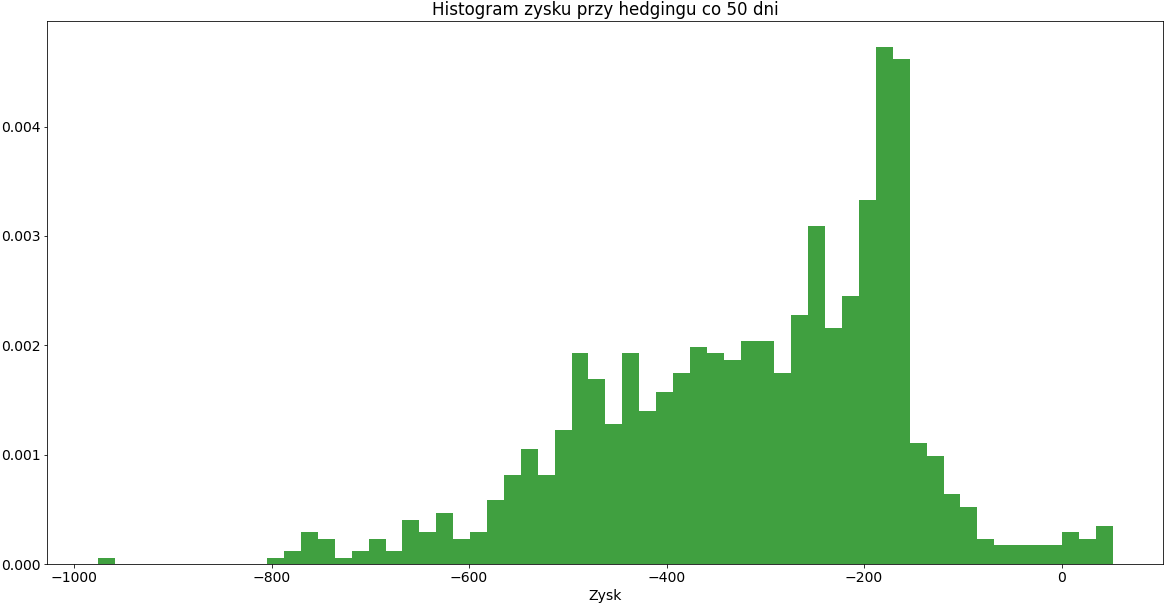
\includegraphics[width=\textwidth,height=\textheight,keepaspectratio]{multi_hedg_f50_dif12.png}
    \caption{Histogram zysków przy zastosowaniu hedgingu trzema opcjami}
    \label{fig:hist_multi_gamma_12_50}
\end{figure}
\end{document}
